\section{实验结果与分析}
在算法实验的过程中,通常先运行一次基础版训练和评估作为基准,然后在此基础上进行优化。这里采用开悟平台提供的框架代码中的默认实现作为基准。
\subsection{基准实验}
为了方便实验中对代码进行改动,采用现有PPO算法的代码作为基础。将PPO算法目录中的代码文件拷贝到diy目录中进行覆盖,然后修改代码文件中导入时的包名称。在提交训练任务时选择diy算法,进行10小时训练,训练结果的模型作为基准模型。为了便于后续对比,基准模型的训练对手采用common\_ai,后期可以清楚的观察到模型的收敛时间和胜率变化等现象。

\imagefigure[1.0]{base_result.png}{base_result}{基准实验的评估结果}
如 \cref{fig:base_result} 所示,即使在自对弈模式下,红蓝双方的结果数据也并不会完全一致。由于双方都是依据环境动态决策,当其中一方先做决策后,另一方会采用不同的策略。回顾游戏视频可以发现,英雄角色在对战中会出现越过兵线,抗兵,抗塔等现象;另外一些时间段会出现英雄没有任何进攻或防御行为,脱离或远离战斗区域,浪费了成长机会;最后,英雄在血量较低的时候,没有后退或者躲避伤害的行为,知道英雄死亡。这些行为也是符合预期的,在后续的优化中,会针对这些问题进行修改。

\imagefigure{base_monitor.png}{base_monitor}{基准训练监控数据}
如 \cref{fig:base_monitor} 所示,从监控面板可以看到,奖励曲线基本在稳定的上升,但是中间也会出现较大的波动,这比较符合基于策略的强化学习模式,通常有较大的方差比较难收敛,而TRPO和PPO就是为了解决方差大和收敛慢的问题。后续可以考虑调整学习率和截断参数的,来验证收敛速度和方差问题。

\imagefigure{base_monitor2.png}{base_monitor2}{基准训练监控比分数据}
如 \cref{fig:base_monitor2} 所示,观察监控中的胜率和防御塔血量数据可以发现,在训练开始后大约5小时,胜率和敌方防御塔血量基本已经稳定,这说明模型已经基本收敛。在后续的训练中,己方防御塔剩余血量继续增加,说明智能体后续的训练在持续的提高己方优势,只是由于对手太弱,已经无法表现在胜率上。

\subsection{修改奖励函数}
智能体决策1V1实验中可以加载已有的模型进行继续训练,这为智能体模型优化提供了便利,可以针对当前模型的问题进行优化然后进行增量训练。按照前面实验设计中设计的奖励函数进行修改后,并将模型的保存时间修改为600秒,即每十分钟保存一个模型,在模型的优化时通常采用较短的保存时间。在基准模型的基础上训练2小时。

\imagefigure{reward_monitor.png}{reward_monitor}{修改奖励函数后的训练过程监控}
如 \cref{fig:reward_monitor} 所示,可以看到在两个小时的训练时间内,reward 略有上升。策略和价值整体波动变化不明显。

\imagefigure{reward_monitor2.png}{reward_monitor2}{修改奖励函数后的训练过程比分监控}
观察训练过程中的对战数据可以发现,在保持胜率的基础上,帧数有稳定的下降趋势,即结束游戏回合所用的时间变短,平均每帧的经济也有下降, 如 \cref{fig:reward_monitor2} 所示。这说明修改的奖励函数产生了效果,英雄更注重尽快结束游戏对战,而不是专注于发展经济和提升等级。

\subsection{修改学习策略}

针对PPO算法的学习策略,验证裁剪范围的影响,和分阶段训练的效果。

\subsubsection{PPO截断}
开悟平台上智能体决策1V1实验代码框架中初始配置的PPO裁剪范围是 0.2 ,训练效果为基准实验中所示。通过将裁剪范围修改为0.3,其他部分保持和基准实验一致,从头开始进行10小时训练。

\imagefigure{clip_result.png}{clip_result}{PPO裁剪范围0.3的训练监控}
如 \cref{fig:clip_result} 所示,修改PPO裁剪范围为 0.3 后,可以看到 reward 和 value\_loss 波动更明显,方差变大,这点符合PPO裁剪变化的预期。总体上模型的训练过程仍然是收敛的,没有出现崩溃现象。

\begin{figure}[htbp]
    \centering
    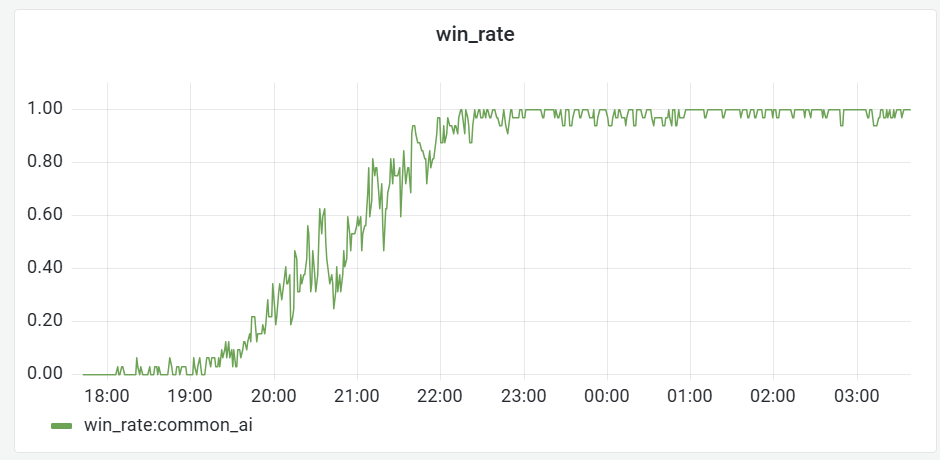
\includegraphics[width=0.6\textwidth]{base_win_rate.png} \\
    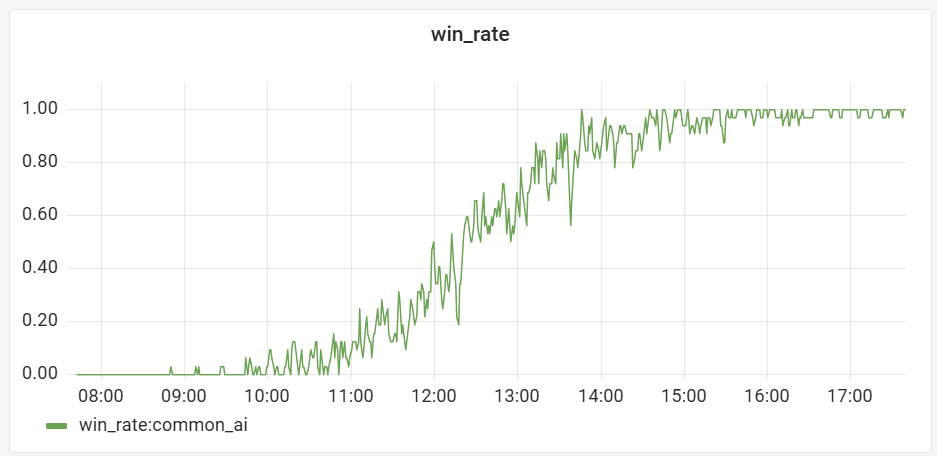
\includegraphics[width=0.6\textwidth]{clip_win_rate.png}
    \caption[short]{PPO裁剪范围0.2(上)和裁剪范围0.3(下)的胜率对比}
    \label{fig:win_rate_diff}
\end{figure}

对比基准实验和本次实验的胜率变化,可以看到PPO裁剪范围0.2的时候,训练过程大约在 $4 \sim 5$ 小时收敛,而PPO裁剪范围0.3的时候,训练过程大约在 7小时收敛,如 \cref{fig:win_rate_diff} 所示。PPO裁剪范围变大的情况下,训练过程比较激进,导致收敛速度较慢。

\imagefigure{clip_eval.png}{clip_eval}{PPO裁剪参数0.3的评估结果}
将本次实验的最终模型提交到模型管理后,进行评估,对手选择为基准实验生成的模型。从结果来看,相对于基准模型,胜率、击杀、经验和金钱均有略微优势,如\cref{fig:clip_eval} 所示。这是由于PPO裁剪范围较大时,训练时可以探索更多的策略,这也导致训练过程收敛较慢。

\subsubsection{分阶段奖励}
从训练过程中来看,训练初期,智能体主要学习如何控制英雄走向中央广场,并在战斗前停止在中央广场的合适的位置。此后,训练智能体控制英雄寻找并攻击敌方阵营和躲避敌方攻击。最后,训练智能体选择合适的攻击目标和取胜策略。

本次实验中,通过先从初始化模型开始,连续训练10小时,得到一个基本的模型,该模型主要学习英雄移动和攻击等基本行为。在此模型的基础上,训练智能体控制英雄角色选择合适的攻击目标,躲避敌方伤害等较高逻辑等级的行为。通常基础训练需要较长时间才能收敛,而后续的优化训练可以使用较高的奖励,快速实现优化模型的效果。本次实验中优化训练选择2小时,从评估结果的录像回放中能看到,英雄已经具有较高的逻辑行为表现。